\subsection{圆柱、圆锥、圆台}\label{subsec:2-4}

\begin{enhancedline}

\subsubsection{圆柱、圆锥、圆台的概念和性质}

圆钢呈圆柱形,铅锤呈圆锥形,粮囤呈圆台形(图 \ref{fig:ltjh-2-30}),这样形状的物体是很多的。

\begin{figure}[htbp]
    \centering
    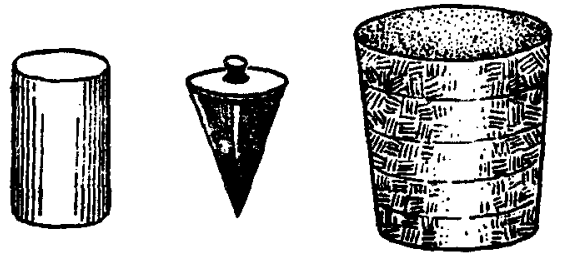
\includegraphics[width=8cm]{../pic/ltjh-ch2-30.png}
    \caption{}\label{fig:ltjh-2-30}
\end{figure}

分别以矩形、直角三角形、直角梯形的一边、一直角边、垂直于底边的腰所在的直线为旋转轴,
其余各边旋转而形成的曲面所围成的几何体分别叫做\zhongdian{圆柱}、\zhongdian{圆锥}、\zhongdian{圆台}(图 \ref{fig:ltjh-2-31})。
旋转轴叫做它们的\zhongdian{轴},在轴上这条边的长度叫做它们的\zhongdian{高},
垂直于轴的边旋转而成的圆面叫做它们的\zhongdian{底面},
不垂直于轴的边旋转而成的曲面叫做它们的\zhongdian{侧面},
无论旋转到什么位置,这条边都叫做\zhongdian{侧面的母线}。
如图 \ref{fig:ltjh-2-31} 中,直线 $O'O$、$SO$ 是轴,线段 $O'O$、$SO$ 是高,$A'A$、$B'B$、$SA$、$SB$ 等是母线。

\begin{figure}[htbp]
    \centering
    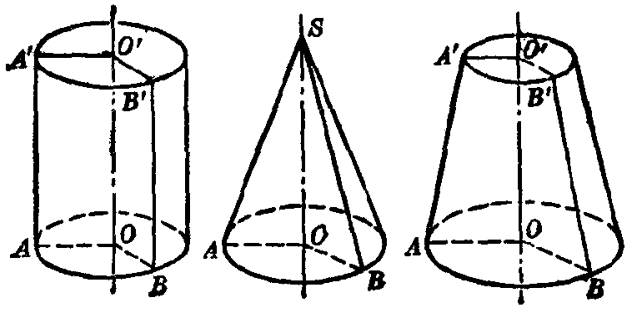
\includegraphics[width=8cm]{../pic/ltjh-ch2-31.png}
    \caption{}\label{fig:ltjh-2-31}
\end{figure}


很明显,圆台也可以看做是用平行于圆锥底面的平面截这个圆锥而得到的。

圆柱、圆锥、圆台用表示它的轴的字母来表示,如圆柱 $O'O$、圆锥 $SO$、圆台 $O'O$。

圆柱、圆锥、圆台有下面的性质:

\zhongdian{(1)平行于底面的截面都是圆;}

\zhongdian{(2)过轴的截面(轴截面)分别是全等的矩形、等腰三角形、等腰梯形。}


\liti 把一个圆锥截成圆台,已知圆台的上、下底面半径的比是 $1:4$,母线长是 10 cm,求圆锥的母线长。

\begin{wrapfigure}[8]{r}{4.5cm}
    \centering
    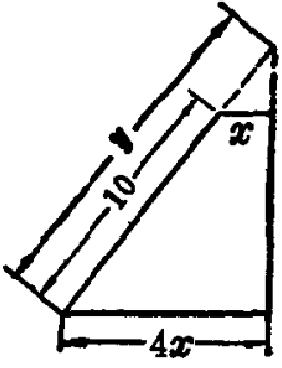
\includegraphics[width=3.5cm]{../pic/ltjh-ch2-32.png}
    \caption{}\label{fig:ltjh-2-32}
\end{wrapfigure}

\jie 设圆锥的母线长为 $y$,圆台上、下底面半径分别是 $x$、$4x$(图 \ref{fig:ltjh-2-32}),根据相似三角形的比例关系,得 \\
\hspace*{10em} $(y-10):y = x:4x$。\\
也就是\\
\hspace*{10em} $4(y-10) = y$,\\
\hspace*{10em} $3y = 40$,

$\therefore$ \quad $y = \dfrac{40}{3}$ (cm)。

因此,圆锥的母线长为 $\dfrac{40}{3}$ cm。


\begin{lianxi}

\xiaoti{用一张 $4 \times 8 \; (\pflm)$ 的矩形硬纸卷成圆柱的侧面。求轴截面的面积(接头忽略不计)。}

\xiaoti{求证:平行于圆锥底面的截面与底面的面积的比,等于顶点到截面的距离与圆锥的高的平方比。}

\xiaoti{圆台侧面的母线长为 $2a$,母线与轴的夹角为 $30^\circ$,一个底面半径是另一个底面半径的 2 倍。求两底面的半径。}

\end{lianxi}


\subsubsection{圆柱、圆锥、圆台的直观图的画法}

圆柱、圆锥、圆台的底面都是圆,圆的直观图,一般不用斜二测画法,而用正等测画法。它的规则是:

\zhongdian{(1)在已知图形 $\yuan\,O$ 中取互相垂直的轴 $Ox$、$Oy$。 画直观图时,
    把它们画成对应的轴 $O'x'$、$O'y'$,使 $\angle x'O'y' = 120^\circ$(或 $60^\circ$)。
}它们确定的平面表示水平平面。

\zhongdian{(2)已知图形上平行于 $x$ 轴或 $y$ 轴的线段,在直观图中,分别画成平行于 $x'$ 轴或 $y'$ 轴的线段。}

\zhongdian{(3)平行于 $x$ 轴或 $y$ 轴的线段,长度都不变。}

下面举例说明这种画法。

\liti 画水平放置的圆的直观图。

\begin{figure}[htbp]
    \centering
    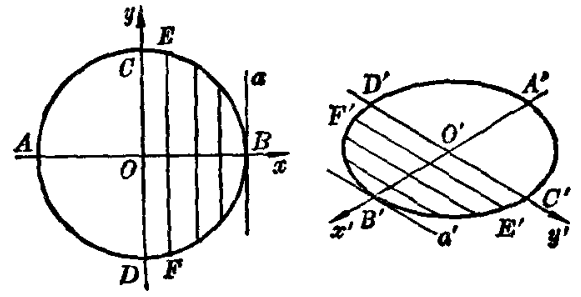
\includegraphics[width=8cm]{../pic/ltjh-ch2-33.png}
    \caption{}\label{fig:ltjh-2-33}
\end{figure}

\huafa (1)如图 \ref{fig:ltjh-2-33},在 $\yuan\,O$ 上取一对互相垂直的直径 $AB$、$CD$,
分别以它们所在的直线作为 $x$ 轴、$y$ 轴。 画对应的 $x'$ 轴、$y'$ 轴,使 $\angle x'O'y' = 120^\circ$。

(2)将 $\yuan\,O$ 的直径 $AB$ 分成 $n$ 等分,过分点画平行于 $y$ 轴的弦 $CD$、$EF$、 …。
在 $x'$ 轴上以 $O'$ 为中点画线段 $A'B'$,使 $A'B' = AB$,
将 $A'B'$ 分成 $n$ 等分,以分点为中点画 $y'$ 轴的平行线段 $C'D'$、$E'F'$、…,
使 $C'D' = CD$, $E'F' = EF$, …。

(3)用平滑曲线顺次连结 $A'$,$D'$,$F'$,$B'$,$E'$,$C'$,…,$A'$,就得到圆的直观图,它是一个椭圆。

我们看到,在这种画法中,圆的中心 $O$,变为椭圆的中心 $O'$,
圆的任意一对互相垂直的直径(如 $AB$、$CD$)变为椭圆的一对直径(如 $A'B'$、$C'D'$),
它们叫做椭圆的\zhongdian{共轭直径}。
圆的切线(如 $a$)变为椭圆的切线(如 $a'$)。

由于椭圆的这种画法比较麻烦,所以实际上通常不用这种画法,而是经过椭圆的一对共轭直径的端点(或再加一点,
如 $E'$)用椭圆模板(图 \ref{fig:ltjh-2-34})来画,或用初中学过的方法画近似椭圆(图 \ref{fig:ltjh-2-35})。

\begin{figure}[htbp]
    \centering
    \begin{minipage}[b]{7cm}
        \centering
        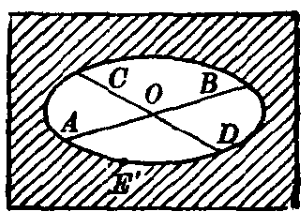
\includegraphics[width=4cm]{../pic/ltjh-ch2-34.png}
        \caption{}\label{fig:ltjh-2-34}
    \end{minipage}
    \qquad
    \begin{minipage}[b]{7cm}
        \centering
        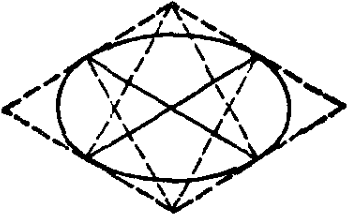
\includegraphics[width=4cm]{../pic/ltjh-ch2-35.png}
        \caption{}\label{fig:ltjh-2-35}
    \end{minipage}
\end{figure}

画圆柱、圆锥、圆台的直观图时,先用上述方法画出底面,其余部分与棱柱、棱锥、棱台直观图的画法类似。下面举例说明它们的画法。


\liti 一个圆锥的底面半径是 1.6 cm,在它的内部有一个底面半径为 0.7 cm,高为 1.5 cm 的内接圆柱\footnotemark。
画出它们的直观图。
\footnotetext{圆柱的下底在圆锥的底面上,上底的圆周在圆锥的侧面上。}

\begin{figure}[htbp]
    \centering
    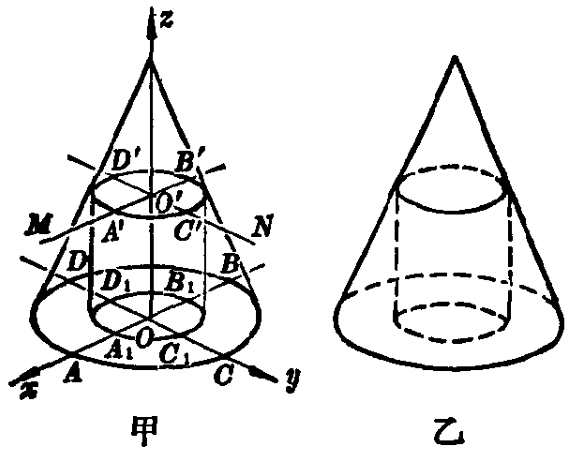
\includegraphics[width=9cm]{../pic/ltjh-ch2-36.png}
    \caption{}\label{fig:ltjh-2-36}
\end{figure}

\huafa (1)画轴 \quad 取 $x$ 轴、$y$ 轴、$z$ 轴,使它们两两相交成 $120^\circ$ 角(图 \ref{fig:ltjh-2-36} 甲)。

(2)画底面 \quad 以 $O$ 为中心,按 $x$ 轴、$y$ 轴画半径等于 1.6 cm 的圆的直观图。

(3)画内接圆柱 \quad 以 $O$ 为中心,按 $x$ 轴、$y$ 轴画一个半径等于 0.7 cm 的圆的直观图,然后在 $z$ 轴上,
取线段 $OO' = 1.5$ cm,过点 $O'$ 作 $O'M \pingxing x \;\text{轴}$, $O'N \pingxing y \;\text{轴}$,
再以 $O'$ 为中心,按 $O'M$、$O'N$ 画一个半径相同的圆的直观图。画圆柱的两条母线,使它们与这两个椭圆相切。

(4)成图 \quad 画圆锥的两条 母线与椭圆 $ACB$ 和 $A'C'B'$ 相切,再加以整理,就得到所要画的直观图(图 \ref{fig:ltjh-2-36} 乙)。


\begin{lianxi}

    画一个上底半径为 1.5 cm,下底半径为 2.5 cm,高为 4 cm 的圆台的直观图(比例尺取 $\exdfrac{1}{2}$,不写画法)。

\end{lianxi}



\subsubsection{圆柱、圆锥、圆台的侧面积}

把圆柱、圆锥、圆台的侧面沿着它们的一条母线剪开后展在平面上,展开图的面积就是它们的侧面积。

\begin{figure}[htbp]
    \centering
    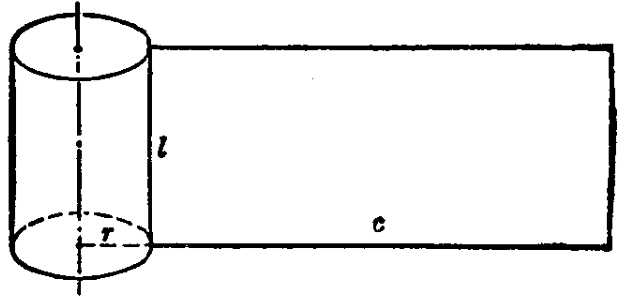
\includegraphics[width=8cm]{../pic/ltjh-ch2-37.png}
    \caption{}\label{fig:ltjh-2-37}
\end{figure}

图 \ref{fig:ltjh-2-37} 是圆柱的侧面展开图,它是一个矩形,这个矩形的长等于圆柱底面周长 $c$,
宽等于圆柱侧面的母线长 $l$ (也是高)。 由此可得:

\begin{dingli}[定理][dl:yzhu-cmj]
    如果圆柱底面半径是 $\bm{r}$,周长是 $\bm{c}$,侧面母线长是 $\bm{l}$,那么它的侧面积是
    \begin{center}
        \framebox[13em]{$\bm{S_\text{圆柱侧} = c\,l = 2\pi rl}$。}
     \end{center}
\end{dingli}

图 \ref{fig:ltjh-2-38} 是圆锥的侧面展开图,它是一个扇形。这个扇形的弧长等于圆锥底面的周长 $c$,
半径等于圆锥侧面的母线长 $l$,由此可得:

\begin{dingli}[定理][dl:yzhui-cmj]
    如果圆锥底面半径是 $\bm{r}$,周长是 $\bm{c}$,侧面母线长是 $\bm{l}$,那么它的侧面积是
    \begin{center}
        \framebox[13em]{$\bm{S_\text{圆锥侧} = \exdfrac{1}{2}c\,l = \pi rl}$。}
     \end{center}
\end{dingli}

\begin{figure}[htbp]
    \centering
    \begin{minipage}[b]{7cm}
        \centering
        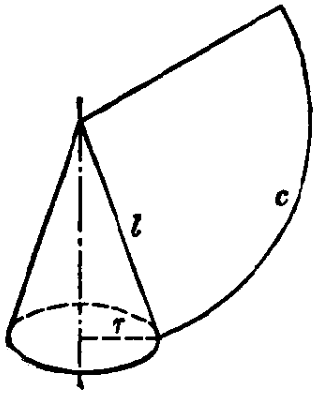
\includegraphics[width=4cm]{../pic/ltjh-ch2-38.png}
        \caption{}\label{fig:ltjh-2-38}
    \end{minipage}
    \qquad
    \begin{minipage}[b]{7cm}
        \centering
        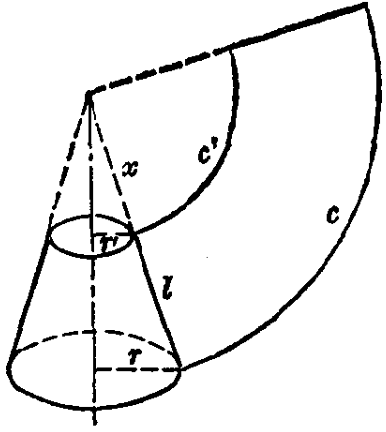
\includegraphics[width=4cm]{../pic/ltjh-ch2-39.png}
        \caption{}\label{fig:ltjh-2-39}
    \end{minipage}
\end{figure}

图 \ref{fig:ltjh-2-39} 是圆台的侧面展开图,通常把这样的图形叫做扇环。 由扇环可以求出圆台的侧面积。

设圆台侧面的母线长为 $l$,上、下底面周长分别是 $c'$、$c$,半径分别是 $r'$、$r$,于是
\begin{gather}
    S_\text{圆台侧} = \exdfrac{1}{2}c \, (l + x) - \exdfrac{1}{2}c'x = \exdfrac{1}{2}[c\,l + (c - c')x] \juhao \tag{1}
\end{gather}

$\because$ \quad $\dfrac{c'}{c} = \dfrac{x}{x + l}$,

$\therefore$ \quad $x = \dfrac{c'l}{c - c'}$。\\
代入 (1),得

$\begin{aligned}
    S_\text{圆台侧} &= \exdfrac{1}{2}\left[ c\,l + (c - c') \dfrac{c'l}{c - c'} \right] \\
        &= \exdfrac{1}{2}(c + c')\,l \\
        &= \pi (r + r')\,l \juhao
\end{aligned}$



由此我们得到下面的定理:

\begin{dingli}[定理][dl:yt-cmj]
    如果圆台的上、下底面半径是 $\bm{r'}$、$\bm{r}$,周长是 $\bm{c'}$、$\bm{c}$,侧面母线长是 $\bm{l}$,那么它的侧面积是
    \begin{center}
        \framebox[18em]{$\bm{S_\text{圆台侧} = \exdfrac{1}{2} (c + c') \,l = \pi (r + r') \,l}$。}
     \end{center}
\end{dingli}

圆柱、圆锥、圆台的全面积,分别等于它们的侧面积与底面积的和。


\liti 已知一个圆锥的底面半径为 $R$,高为 $H$。在其中有一个高为 $x$ 的内接圆柱。

(1)求圆柱的侧面积;(2) $x$ 为何值时,圆柱的侧面积最大?

\jie (1)画圆锥及内接圆柱的轴截面(图 \ref{fig:ltjh-2-40})。 设所求的圆柱的底面半径为 $r$,它的侧面积
$$ S_\text{圆柱侧} = 2\pi rx \juhao $$

$\because$ \quad $\exdfrac{r}{R} = \dfrac{H - x}{H}$,(为什么?)

$\therefore$ \quad $r = R - \exdfrac{R}{H} \cdot x$。

$\therefore$ \quad $S_\text{圆柱侧} = 2\pi Rx - \dfrac{2\pi R}{H} \cdot x^2$。


(2)因为 $S_\text{圆柱侧}$ 的表示式中 $x^2$ 的系数小于零,所以这个二次函数有最大值。
这时圆柱的高是
$$ x = -\dfrac{2\pi R}{-2 \cdot \dfrac{2\pi R}{H}} = \exdfrac{H}{2} \juhao $$

当圆柱的高是已知圆锥的高的一半时,它的侧面积最大。

\begin{figure}[htbp]
    \centering
    \begin{minipage}[b]{7cm}
        \centering
        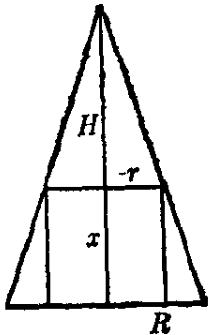
\includegraphics[width=4cm]{../pic/ltjh-ch2-40.png}
        \caption{}\label{fig:ltjh-2-40}
    \end{minipage}
    \qquad
    \begin{minipage}[b]{7cm}
        \centering
        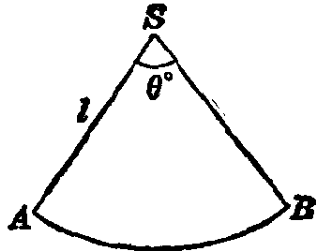
\includegraphics[width=5cm]{../pic/ltjh-ch2-41.png}
        \caption{}\label{fig:ltjh-2-41}
    \end{minipage}
\end{figure}

\liti 圆锥的底面半径为 $r$,侧面母线长为 $l$,侧面展开图扇形的圆心角为 $\theta^\circ$。
求证: $\theta = \exdfrac{r}{l} \cdot 360$ (度)。

\zhengming 图 \ref{fig:ltjh-2-41} 是圆锥侧面展开图。因为扇形的弧长等于圆锥底面的周长,即 \\
\hspace*{10em} $\dfrac{\pi\, l\, \theta}{180} = 2\pi r$。 \\
所以 \hspace{8em} $\theta = \exdfrac{r}{l} \cdot 360$ (度)。

在圆台的侧面积公式中,
如果设 $c' = c$,就得到圆柱侧面积公式: $S_\text{圆柱侧} = c \, l$。
如果设 $c' = 0$,就得到圆锥侧面积公式: $S_\text{圆锥侧} = \exdfrac{1}{2} c \, l$。
这样,圆柱、圆锥、圆台的侧面积公式之间的关系可表示如下图。

\begin{figure}[htbp]
    \centering
    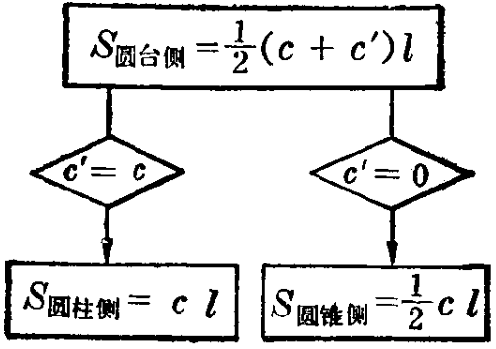
\includegraphics[width=7cm]{../pic/ltjh-ch2-subsec4-gsgx.png}
\end{figure}

\begin{lianxi}

\xiaoti{将半径为 $r$ 的薄铁圆板沿三条半径截成全等的三个扇形,做成三个圆锥筒。求圆锥筒的高(不计接头)。}

\xiaoti{一个直角梯形的上、下底和高的比为 $1:2:\sqrt{3}$。 求它旋转而成的圆台的上底面积、下底面积和侧面积的比。}

\xiaoti{把圆柱、圆锥、圆台的侧面积用中截面周长及母线长表示出来。}

\end{lianxi}

\end{enhancedline}

